\documentclass[border=4pt]{standalone}

\usepackage{amsmath}
\usepackage{tikz}
\usepackage{mathdots}
\usepackage{yhmath}
\usepackage{cancel}
\usepackage{color}
\usepackage{siunitx}
\usepackage{array}
\usepackage{multirow}
\usepackage{amssymb}
\usepackage{gensymb}
\usepackage{tabularx}
\usepackage{booktabs}
\usetikzlibrary{fadings}
\usetikzlibrary{patterns}


\begin{document}

\tikzset{every picture/.style={line width=0.75pt}} %set default line width to 0.75pt

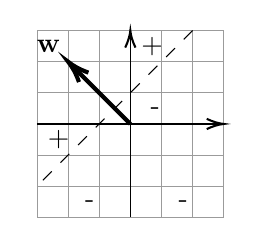
\begin{tikzpicture}[x=0.75pt,y=0.75pt,scale=0.75,yscale=-1,xscale=1]
    %uncomment if require: \path (0,362.03123474121094); %set diagram left start at 0, and has height of 362.03123474121094

    %Shape: Grid [id:dp41292874782543265]
    \draw  [draw opacity=0][line width=0.25]  (210,100) -- (330,100) -- (330,220) -- (210,220) -- cycle ; \draw  [color={rgb, 255:red, 155; green, 155; blue, 155 }  ,draw opacity=1 ][line width=0.25]  (230,100) -- (230,220)(250,100) -- (250,220)(270,100) -- (270,220)(290,100) -- (290,220)(310,100) -- (310,220) ; \draw  [color={rgb, 255:red, 155; green, 155; blue, 155 }  ,draw opacity=1 ][line width=0.25]  (210,120) -- (330,120)(210,140) -- (330,140)(210,160) -- (330,160)(210,180) -- (330,180)(210,200) -- (330,200) ; \draw  [color={rgb, 255:red, 155; green, 155; blue, 155 }  ,draw opacity=1 ][line width=0.25]  (210,100) -- (330,100) -- (330,220) -- (210,220) -- cycle ;
    %Straight Lines [id:da2811722352478421]
    \draw [line width=1.5]    (270,160) -- (232.12,122.12) ;
    \draw [shift={(230,120)}, rotate = 405] [color={rgb, 255:red, 0; green, 0; blue, 0 }  ][line width=1.5]    (14.21,-4.28) .. controls (9.04,-1.82) and (4.3,-0.39) .. (0,0) .. controls (4.3,0.39) and (9.04,1.82) .. (14.21,4.28)   ;

    %Straight Lines [id:da558647267855283]
    \draw  [dash pattern={on 4.5pt off 4.5pt}]  (310,100) -- (210,200) ;


    %Straight Lines [id:da47605194626185665]
    \draw    (210,160) -- (328,160) ;
    \draw [shift={(330,160)}, rotate = 180] [color={rgb, 255:red, 0; green, 0; blue, 0 }  ][line width=0.75]    (10.93,-3.29) .. controls (6.95,-1.4) and (3.31,-0.3) .. (0,0) .. controls (3.31,0.3) and (6.95,1.4) .. (10.93,3.29)   ;

    %Straight Lines [id:da09041975422816395]
    \draw    (270,220) -- (270,102) ;
    \draw [shift={(270,100)}, rotate = 450] [color={rgb, 255:red, 0; green, 0; blue, 0 }  ][line width=0.75]    (10.93,-3.29) .. controls (6.95,-1.4) and (3.31,-0.3) .. (0,0) .. controls (3.31,0.3) and (6.95,1.4) .. (10.93,3.29)   ;


    % Text Node
    \draw (217.5,110) node   [align=left] {$\mathbf{w}$};
    % Text Node
    \draw (224,170) node   [align=left] {+};
    % Text Node
    \draw (284,110) node   [align=left] {+};
    % Text Node
    \draw (304,210) node   [align=left] {\mbox{-}};
    % Text Node
    \draw (286,150) node   [align=left] {\mbox{-}};
    % Text Node
    \draw (244,210) node   [align=left] {\mbox{-}};


\end{tikzpicture}

\end{document}
